%% The Discrete Fourier transform

\subsection*{The Discrete Frequency Domain}


    \begin{figure}[htb]
        \begin{center}
            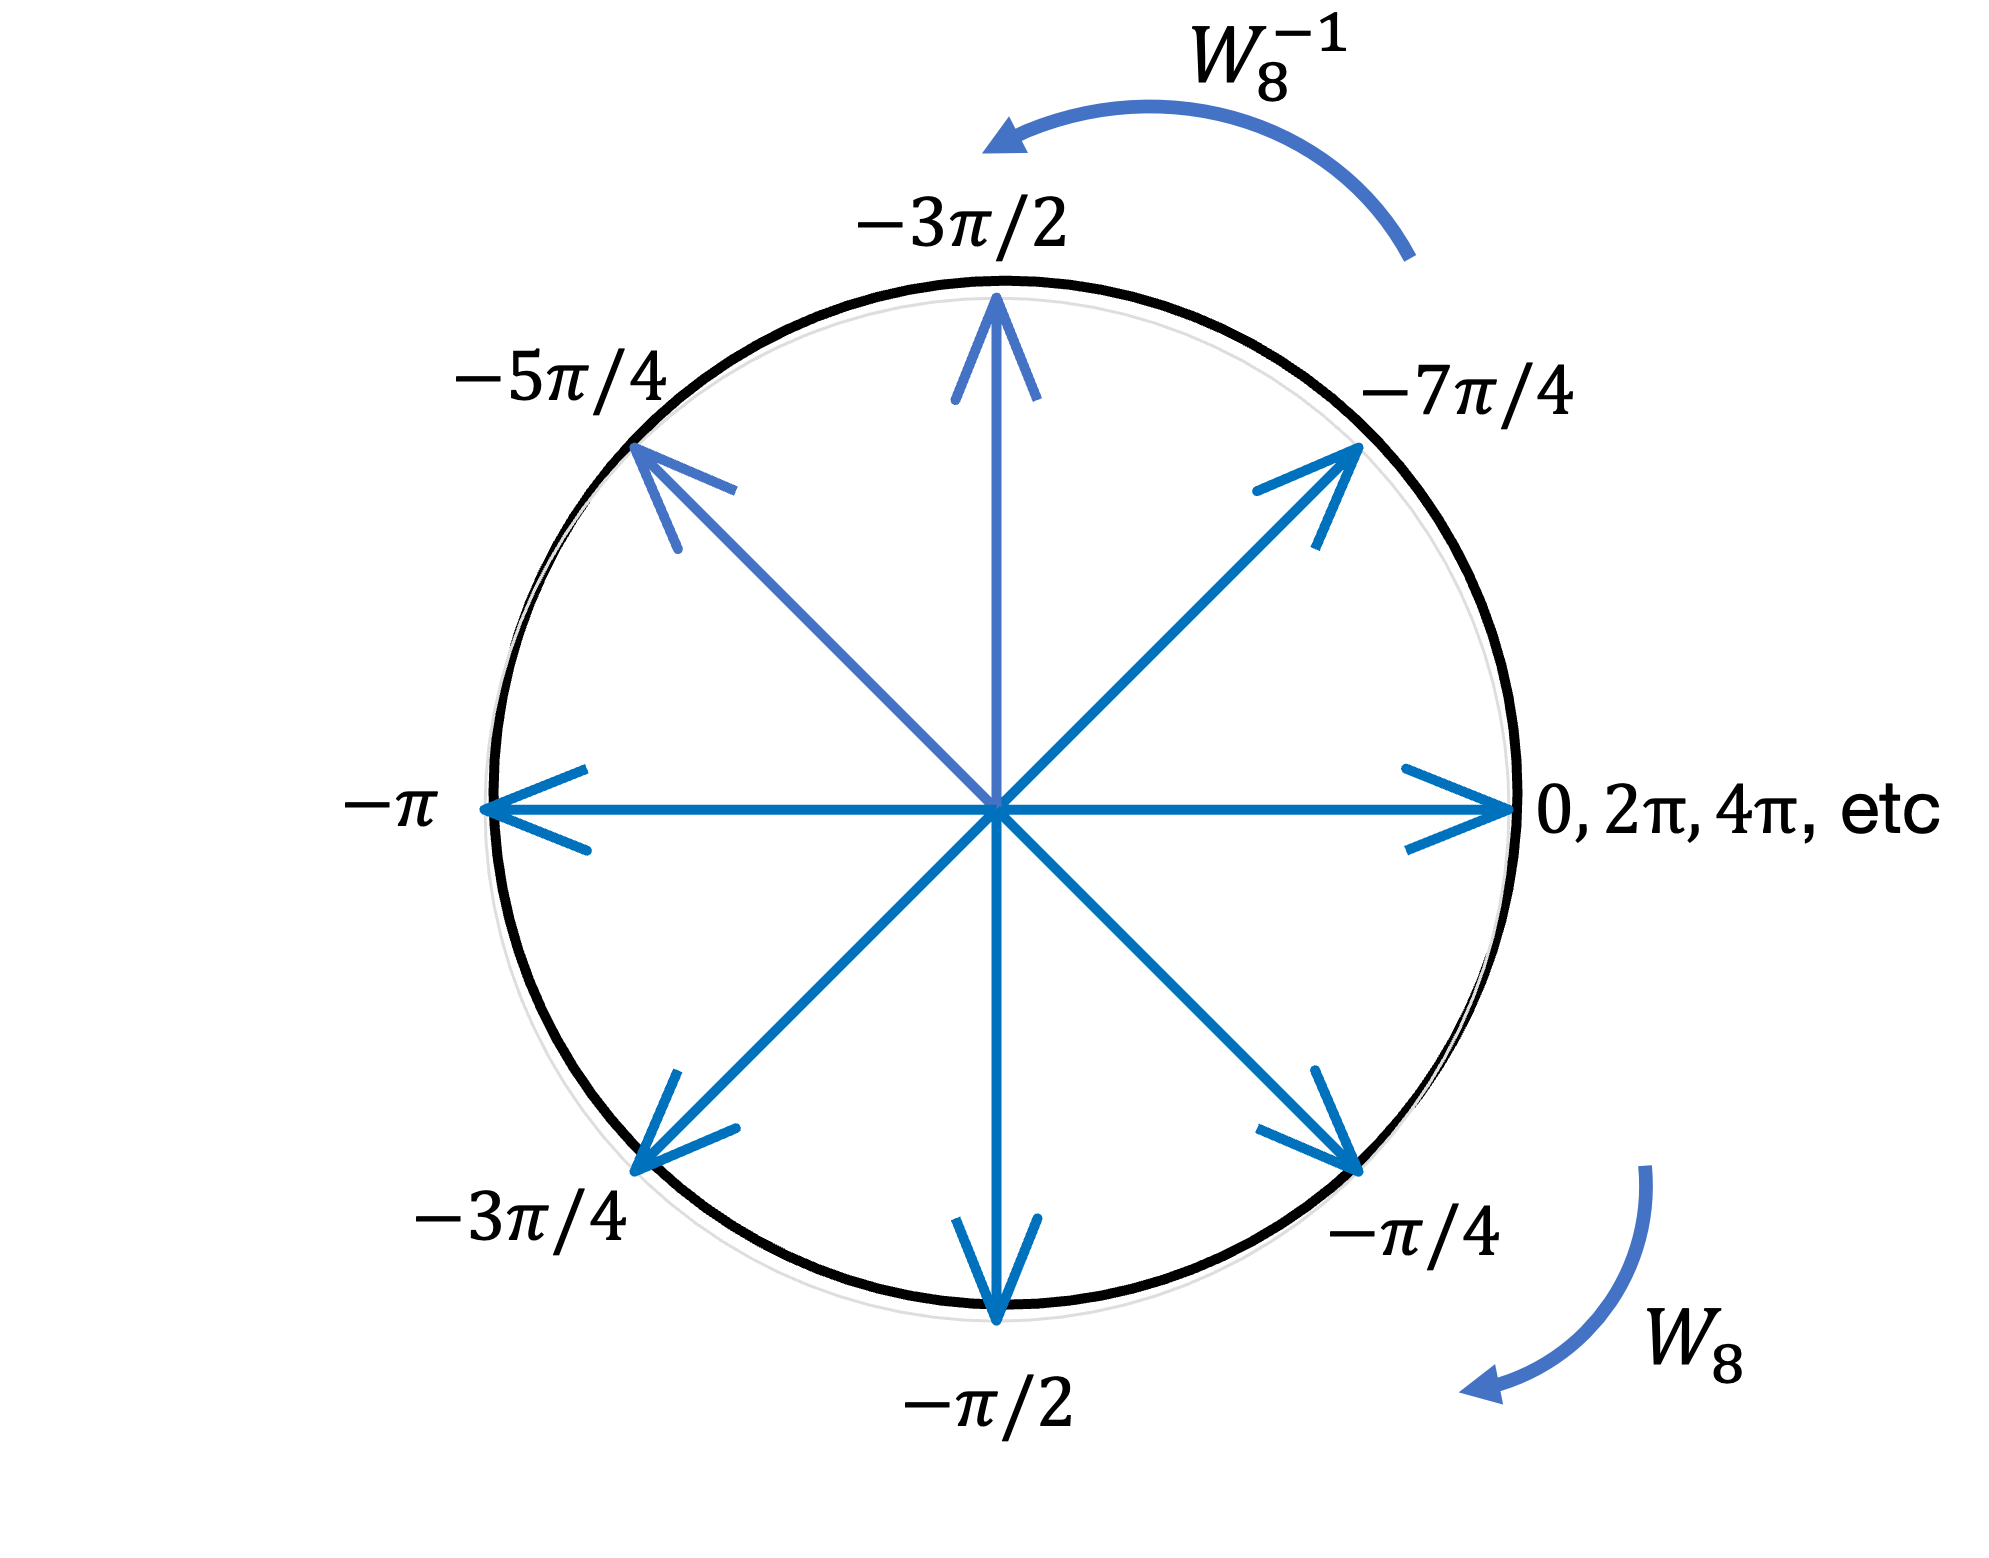
\includegraphics[width=0.5\textwidth]{formula-sheets/w_wheel.png}
            \caption{\label{fig:w_wheel} The function $W_8$ and $W_8^{-1}$}
        \end{center}
    \end{figure}



\subsubsection*{The Discrete Fourier Transform}

$$
X[m] = \sum_{n=0}^{N-1} x[n] W_N^{nm}
$$
where $W_N = \exp\left(-\frac{j2\pi}{N}\right)$.

\subsubsection*{The Inverse Discrete Fourier Transform}

$$
x[n] = \sum_{m=0}^{N-1}  x[m]W_N^{-nm}
$$
where $W_N^{-1}=\exp\left(\frac{j2\pi}{N}\right)$.

\subsection*{The function $W_N$}

$$
W_N = \exp\left(\frac{j2\pi}{N}\right) %
     = \cos\left(\frac{2\pi}{N}\right)+j\sin\left(\frac{2\pi}{N}\right)
$$
The functions $W_N$ and $W_N^{-1}$ are illustrated in Fig.~\ref{fig:w_wheel} for $N = 8$.

\endinput

